\chapter{MARCO TEÓRICO}

\section{Conceptos de código fuente}

\subsection{Lenguaje de programación}
Los lenguajes de programación son notaciones que describen los cálculos a las personas y las máquinas. Nuestra percepción del mundo en que vivimos depende de los lenguajes de programación, ya que todo el software que se ejecuta en todas las computadoras se escribió en algún lenguaje de programación \cite{aho2008compiladores}.

Un lenguaje de programación es un lenguaje formal, que mediante un conjunto de instrucciones permite a un programador crear programas. El lenguaje de programación es un sistema estructurado de comunicación conformado por conjuntos de símbolos, palabras clave, reglas semánticas y sintácticas, las cuales sirven para el entendimiento entre un programador y una maquina.

\subsection{Código fuente}
En informática, se denomina código fuente a la conjunto de lineas de texto que escritas por un programador. Estas lineas de texto representan instrucciones en un lenguaje de programación. Las instrucciones representan los pasos que debe seguir la computadora para la ejecución de un programa específico.

El código fuente no es directamente ejecutable por la computadora, este debe ser traducido a otro lenguaje de modo que la computadora pueda interpretarlo. En la traducción se usan compiladores, ensambladores, interpretes y otros.

\subsection{Ofuscación de código fuente}
Según \cite{wiki:Plagiarism} la Real Academia Española define como plagio a la acción de copiar en lo sustancial obras ajenas, dándolas como propias. El plagio de código fuente consiste en utilizar el código fuente de otra persona y adjudicarse como propio.
La ofuscación se refiere a encubrir el significado de una comunicación haciéndola más confusa y complicada de interpretar \cite{wiki:Obfuscation_(software)}.

En computación, la ofuscación se refiere al acto deliberado de realizar un cambio no destructivo, ya sea en el código fuente de un programa informático, en el código intermedio (bytecodes) o en el código máquina cuando el programa está en forma compilada o binaria. Es decir, se cambia el código se enrevesa manteniendo el funcionamiento original, para dificultar su entendimiento. De esta forma se dificultan los intentos de ingeniería inversa y desensamblado que tienen la intención de obtener una forma de código fuente cercana a la forma original \cite{wiki:Obfuscation_(software)}.

\subsection{Métodos de ofuscación de código fuente}
Existen muchos métodos de ofuscación utilizados por estudiantes para ocultar la similitud a continuación se mencionan algunos:
\begin{itemize}
    \item \cite{article3} Mencionan cambios visuales en el formato del código, por lo que parece diferente a primera vista, esto generalmente incluye la modificación de espacios en blanco como sangrías, espacios, nuevas líneas, etc.
    \item \cite{article3} Mencionan cambios en los comentarios del código.
    \item \cite{donaldson1981plagiarism} Mencionan el cambio de los nombres de los identificadores. como nombres de variables, nombres de constantes, nombres de funciones, nombres de clases, etc.
    \item \cite{donaldson1981plagiarism} Mencionan reordenar las líneas del código para las que el pedido no marca ninguna diferencia. Estos incluyen cambiar el orden de las declaraciones de variables, cambiando el orden de las declaraciones dentro de bloques de código como funciones, re ordenación de bloques de código o funciones, re ordenación de clases internas, etc.
\end{itemize}

\section{Conceptos de compiladores}

\subsection{Procesador de lenguaje}
Un procesador de lenguaje se muestra en la figura \ref{compilador1}. También llamado compilador es un programa que puede leer un programa en un lenguaje y traducirlo en un programa equivalente en otro lenguaje. Una función importante del compilador es reportar cualquier error en el programa fuente que detecte durante el proceso de traducción \cite{aho2008compiladores}.
\begin{figure}[h!]
\centering
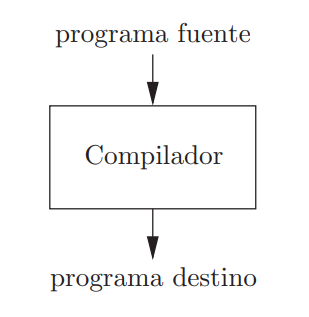
\includegraphics[scale=0.6]{imagenes/compilador1}
\caption{Un compilador}
Nota: Figura tomada de \cite{aho2008compiladores}.
\label{compilador1}
\end{figure}

El proceso de compilación opera como una secuencia de fases con las cuales transforma un programa fuente en otro, se muestra en la figura \ref{fasesCompilador1}.
\begin{figure}[h!]
\centering
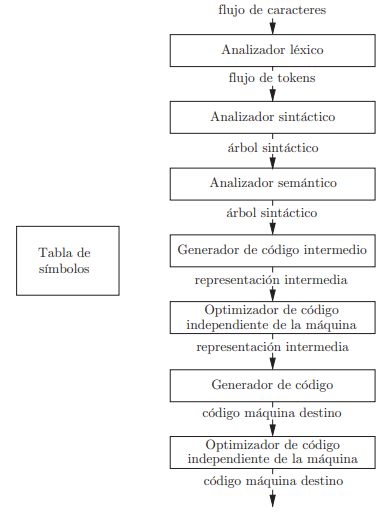
\includegraphics[scale=1]{imagenes/fasesCompilador1}
\caption{Fases de un compilador}
Nota: Figura tomada de \cite{aho2008compiladores}.
\label{fasesCompilador1}
\end{figure}

En el presente trabajo de investigación, solo es de interés de cubrir los teoría y conceptos hasta el análisis semántico.

\subsection{Análisis Léxico}
\cite{aho2008compiladores} Explica que la primera fase de un compilador se le llama análisis léxico o escaneo. El analizador léxico lee el flujo de caracteres que componen el programa fuente y los agrupa en secuencias significativas, conocidas como lexemas. Para cada lexema, el analizador léxico produce como salida un token. Estos lexemas son los que pasaran a la siguiente fase, el análisis de la sintaxis. El analizador léxico ignora los espacios en blanco que separan los lexemas.\\

\cite{catalan2010compiladores} Explica que esta fase consiste en leer el texto del código fuente carácter a carácter e ir generando los tokens. Estos tokens constituyen la entrada para el siguiente proceso de análisis. El agrupamiento de caracteres en tokens depende del lenguaje que vayamos a compilar. Es decir un lenguaje generalmente agrupara caracteres en tokens diferentes de otro lenguaje. Los tokens pueden ser de dos tipos, cadenas específicas como palabras reservadas, puntos y comas, etc., y no específicas, como identificadores, constantes y etiquetas. La
diferencia entre ambos tipos de tokens radica en si ya son conocidos previamente o no. El analizador léxico irá ignorando las partes no esenciales para la siguiente fase, como pueden ser los espacios en blanco, los comentarios, etc., es decir, realiza la función de preprocesador en cierta medida. Por lo tanto, y resumiendo, el analizador léxico lee los caracteres que componen el texto del programa fuente y suministra tokens al analizador sintáctico.

\subsection{Análisis Sintáctico}
\cite{aho2008compiladores} Explica que la segunda fase del compilador es el análisis sintáctico o parsing. El parser utiliza los primeros componentes de los tokens producidos por el analizador de léxico para crear una representación intermedia en forma de árbol que describa la estructura gramatical del flujo de tokens. Una representación típica es el árbol sintáctico, en el cual cada nodo interior representa una operación y los hijos del nodo representan los argumentos de la operación. En la figura \ref{traduccion1} se muestra un árbol sintáctico para el flujo de tokens como salida del analizador sintáctico.\\

\cite{catalan2010compiladores} Explica que el analizador sintáctico tiene como entrada los lexemas que le suministra el analizador léxico y su función es comprobar que están ordenados de forma correcta dependiendo del lenguaje que se quiere procesar. Los dos analizadores suelen trabajar
unidos e incluso el léxico suele ser una subrutina del sintáctico. El analizador sintáctico se le suele llamar parser, este genera de manera teórica un árbol sintáctico. Este árbol se puede ver como una estructura jerárquica que para su construcción se usa reglas recursivas. La estructuración de este árbol hace posible diferenciar entre aplicar unos operadores antes de otros en la evaluación de expresiones. En resumen la tarea del analizador sintáctico es procesar los lexemas que le suministra el analizador léxico, comprobar si están bien ordenados, y si no lo están, generar los informes correspondientes. Si la ordenación, se generará un árbol sintáctico teórico.

\subsection{Análisis Semántico}
\cite{aho2008compiladores} Explica que el analizador semántico utiliza el árbol sintáctico y la información en la tabla de símbolos para comprobar la consistencia semántica del programa fuente con la definición del lenguaje. También recopila información sobre el tipo y la guarda, ya sea en el árbol sintáctico o en la tabla de símbolos, para usarla más tarde durante la generación de código intermedio.
Una parte importante del análisis semántico es la comprobación de tipos, en donde el compilador verifica que cada operador tenga operando que coincidan.\\

\cite{catalan2010compiladores} Explica que esta fase toma el árbol sintáctico teórico de la anterior fase y hace una serie de comprobaciones antes de obtener un árbol semántico teórico.
Esta fase es quizás la más compleja. Hay que revisar que los operadores trabajan sobre tipos compatibles, si los operadores obtienen como resultado elementos con tipos adecuados, si las llamadas a subprogramas tienen los parámetros adecuados tanto en
número como en tipo, etc. Esta fase debe preparar el terreno para atajar las fases de generación de código y debe lanzar los mensajes de error que encuentre. En resumen, su tarea es revisar el significado de lo que se va leyendo para ver si tiene sentido.

\begin{figure}[h!]
\centering
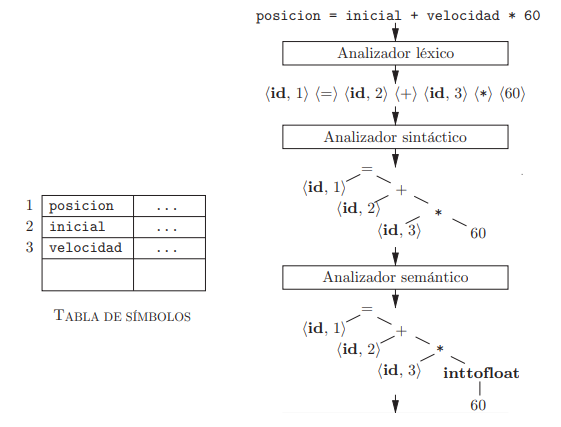
\includegraphics[scale=0.9]{imagenes/traduccionDeAsignacion1}
\caption{Traducción de una asignación}
Nota: Figura tomada de \cite{aho2008compiladores}.
\label{traduccion1}
\end{figure}

\subsection{Árboles de sintaxis abstracta}
\cite{Aho1999} Explica que un árbol es una estructura jerárquica sobre una colección de objetos, como ejemplos están los arboles genealógicos y organigramas. Los arboles son útiles para analizar circuitos eléctricos y para representar estructuras de formulas matemáticas. Dentro de la área de la computación se usan para organizar la información en sistemas de bases de datos y para representar la estructura sintáctica de un programa fuente en compiladores.

En \cite{Cormen2009} podemos obtener una definición y propiedades matemáticas de un árbol, para ello se desarrollaran algunas definiciones de teoría de grafos. Sea G un grafo no direccionado es representado por un par $G=(V,E)$, donde V representa el conjunto de vértices de G, se le denota con un circulo. E representa el conjunto de aristas de G, se le denota con una linea.\\
Ademas para que un grafo sea considerado un árbol deben cumplirse las siguientes afirmaciones:
\begin{itemize}
    \item Dos vértices de G están conectados por un camino único.
    \item G es conexo, pero si se elimina cualquier vértice que no sea una hoja de E, el grafo resultante es no conexo.
    \item G es conexo, y $|E| = |V|-1$.
    \item G es acíclico, y $|E| = |V|-1$.
    \item G es acíclico, pero si cualquier vértice es agregado a E, el grafo resultante contendrá un ciclo.
\end{itemize}
\begin{figure}[h!]
\centering
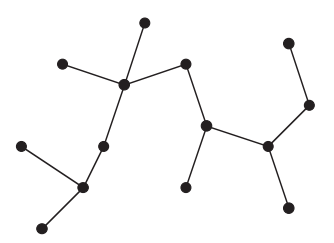
\includegraphics[scale=0.8]{imagenes/arbol1}
\caption{Árbol}
Nota: Figura tomada de \cite{Cormen2009}.
\label{arbol1}
\end{figure}

En resumen un árbol es un grafo no direccionado, conexo, acíclico, y que dos vértices cualesquiera están conectados por un camino único, como se muestra en la figura \ref{arbol1}.

Las estructuras de datos basadas en árboles se hicieron muy populares en el campo del desarrollo de compiladores: cada vez que se envía un archivo que contiene el código fuente al compilador, se realizan varios pasos antes de que se puedan generar las instrucciones de la máquina. El código tiene que ser tokenizado por un Lexer primero: separa el flujo de entrada en tokens individuales y los pasa al analizador, que utiliza una gramática libre de contexto del lenguaje de programación para construir una representación de código intermedio, un llamado árbol de análisis.
Cada token encontrado por el lexer está representado por un nodo en el árbol de análisis. No todos los tokens (nodos) tienen un valor semántico: algunos tokens, por ejemplo, paréntesis y punto y coma, son puramente sintácticos. Por lo tanto, puede omitirse. La estructura de datos resultante se denomina árbol de sintaxis abstracta (AST).
Ahora que el código fuente se representa como un árbol, se puede analizar de una forma más sofisticada manera que al analizar el flujo de token plano: el árbol se puede recorrer o buscar de varias maneras por ejemplo, pos-orden, pre-orden, búsqueda profundidad, etc. \cite{ChangeDistiller}.

\section{Conceptos de algorítmica}

\subsection{Programación dinámica}
La programación dinámica es una técnica matemática que se utiliza para la solución de problemas matemáticos seleccionados, en los cuales se toma un serie de decisiones en forma secuencial.

\subsection{Distancia de edición de árbol}
La distancia edición o distancia entre palabras es el número mínimo de operaciones requeridas para transformar una cadena de caracteres en otra, se usa ampliamente en teoría de la información y ciencias de la computación. Se entiende por operación, bien una inserción, eliminación o la sustitución de un carácter. Esta distancia recibe ese nombre en honor al científico ruso Vladimir Levenshtein, quien se ocupó de esta distancia en 1965. Es útil en programas que determinan cuán similares son dos cadenas de caracteres, como es el caso de los correctores ortográficos.\\

La distancia de edición del árbol se define como la secuencia de costos mínimos de operaciones de edición de nodos que transforman un árbol en otro. Las operaciones consisten en eliminar, agregar y modificar nodos del árbol.

\subsection{Conjuntos Disjuntos}
En \cite{Cormen2009} obtenemos una la definición de conjuntos disjuntos y la estructura de datos para conjuntos disjuntos.

Los conjuntos disjuntos es una colección representada por $S=\{ S_1,S_2,...,S_k \}$ donde cada elemento $S_i$ representa un conjunto dinámico, y para cada elemento de la colección se cumple que $S_i \cap S_j = \emptyset$.

La estructura de datos para conjuntos disjuntos soporta eficientemente las operaciones de crear un conjunto, búsqueda del representante de un conjunto y la unión de conjuntos.

\noindent Sean u y v elementos de un conjunto:
\begin{itemize}
    \item $MAKE-SET(u)$ Crea un nuevo conjunto cuyo único miembro es u. Dado que los conjuntos son disjuntos, es necesario que u no se encuentre en otro conjunto.
    \item $UNION(u, v)$ Une los conjuntos dinámicos que contienen a u y v, es decir $S_u \cap S_v$, el representante del conjunto resultante sera cualquiera de los dos.
    \item $FIND-SET(u)$ devuelve un puntero al representante del conjunto que contiene a u.
\end{itemize}

\section{Herramientas para la detección de similitud de código}
\subsection{Algoritmos utilizados para la detección de similitud}
\cite{10.1145/3313290} Identificó diferentes algoritmos a continuación se mencionan algunos de ellos:
\begin{itemize}
    \item Recuento de atributos
    \item Huella digital
    \item Coincidencia de cadena
    \item Texto base
    \item Estructura base
    \item Estilo
    \item Semántico
    \item N-gramas
    \item Árboles
    \item Grafos
\end{itemize}
Algunos de estos fueron inventados en la década de 1980. También hace mención a que los enfoques basados en estructuras son mucho mejores y que la mayoría de las herramientas de detección de similitud combinan más de un tipo de algoritmo.
\subsection{Detección léxica}
Las técnicas y herramientas para computar las diferencias textuales entre documentos son bien conocidas y aprobadas. Sin embargo, las herramientas existentes como GNU diff tratan con información plana, en lugar de jerárquica. Por lo general, calculan una lista de líneas que deben cambiarse, insertarse o eliminarse para que un primer documento coincida con el segundo. \cite{ChangeDistiller}.